\chapter{Hardware Based Security}
Traditional computing has 6 principle regarding processors designes, which are used to enhance the
performces squeezing the most out of the hardware, which are:
\begin{itemize}
  \item \textbf{caching}, which hides consecutive memory access latency
  \item \textbf{pipelining}, which allows to execute multiple instructions at the same time
  \item \textbf{prediction}, chich allows to guess the control flow direction before it is known
  \item \textbf{parallelizing}, which allows to process multiple data at the same time
  \item \textbf{use of indirection},
  \item \textbf{specialization}, which allows to use specific hardware for specific tasks
\end{itemize}
All those measures allow to increase the performances of the processor, but they also introduce
vulnerabilities, which can be exploited by attackers.  This is because they were introduced without
considering security, and they were designed to be fast, not secure.  

Of course, not all the processor are general purpose ones, and some of them are designed to be
secure, providing extra logical isolation for the software running on them. This is the case of 
\textbf{Secure Processor Architectures}, which extend a processor with hardware (and related
software) features for the protection of software. The protected sofware and data is called
\textbf{enclave}, but this can also be the whole operating system or a virtual machine. This is done
because even if we trust som hardware, we cannot trust all the software running on it,
\textit{never}.\\
The isolation measures should also cover all kinds of possible ways to perform a information leak,
of any kind of information, both at the architectural and microarchitectural level, and from any
hardware component, meaning that everything should be untrusted by default.
\begin{boxH}
  A computer system with no secure components nor secure processor architecture considers all the
  components as trusted, which is \textbf{not} a good idea.
\end{boxH}

\begin{figure}[H]
  \centering
  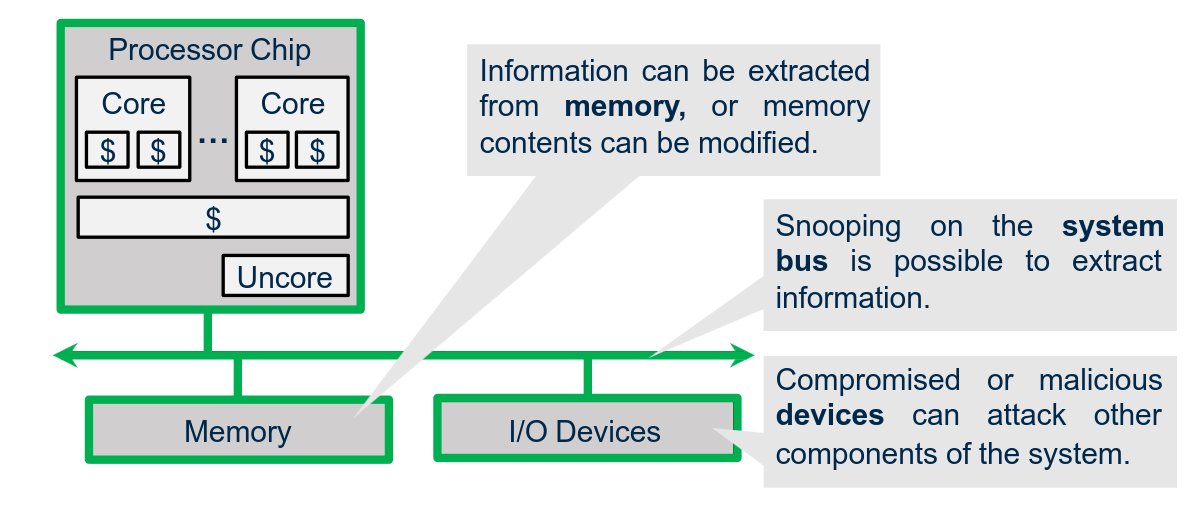
\includegraphics[width=0.7\textwidth]{img/hardware/unsecure processor.png}
  \caption{An example of unsecure processor, with a description of some possible attacks}
\end{figure}

Typically, a computer systen uses a \textbf{ring-based protection scheme}, which gives the most
privileges (and most trust) to the lowest levels of the system software. This means that if the 
lowest level is compromised, the whole system is compromised. Usually, 3 levels are designed:
\begin{itemize}
  \item \textbf{Ring 0}, which is the most privileged level, and is used by the kernel
  \item \textbf{Ring 1 and 1}, which is used by the drivers and other semi-privileged software, but
    it is rarely used
  \item \textbf{Ring 3}, which is used by the applications and us the least privileged level
\end{itemize}
but there are also other levels that can be defined:
\begin{itemize}
  \item \textbf{Ring -1}, which is used by the hypervisor
  \item \textbf{Ring -2}, which is used by the \textbf{System Management Mode} (SMM) and is ussually
    locked down by the processor manifacturer
  \item \textbf{Ring -3}, which is used by the \textbf{Platform management engine} which runs on a
    separate processor
\end{itemize}

\begin{figure}[H]
  \centering
  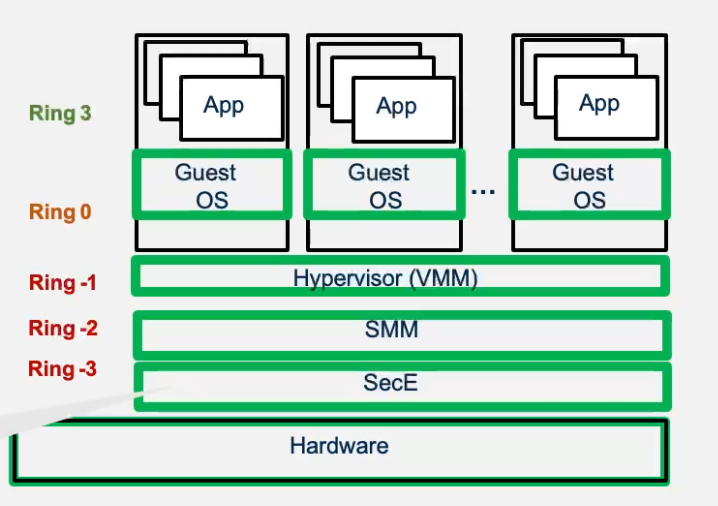
\includegraphics[width=0.5\textwidth]{img/hardware/ring protection scheme.png}
  \caption{The general ring protection scheme}
\end{figure}
In this schema, the relationship between the ring level and the privilege level is inverted, meaning
that the higher the ring level, the lower the privilege level. This schema also guarantees extra
layers of protection to the hardware, which is the most trusted component of the system, but it
instrincaly means that each component trust the lower one.\\
So far we have considered the processor to be secure, which means that we trust it, but the same is
not true for the rest of the hardware, such as the memory or the bus. From those components, threats
can arise, which are \textit{underestimated} when designing a secure processor architecture, part of
those can't even be dealt with in a proper way, for example side channels.
\begin{section}{TEE and TCB}
  \begin{boxH}
    The \textbf{Trusted Computing Base} (TCB) is the set of hardware and software that is
    responsible for realizing the Trusted Execution Environments (TEEs).
  \end{boxH}
  Notice that the goal of TEE is to protect a piece of code and data( in particular the CIA
  proprieties) from a range of software and hardware attacks, for this reason the TCB is trusted to
  implement the protections correctly, meaning that a vulnerability or a successful attack on it
  nullifies the protection on the TEE.\\
  TEE are used to protect different parts of the system according to the architecture, for example
  they can be used to protect either \textit{Trusted Software Modules}(which are the enclaves) or 
  a whole virtual machine.\\

  With the introduction of the TCB, the linear relationship between the ring level and the
  privileged level is broken, because the different hw and software components can be either trusted
  of not by the different components of the TCB.\\
  \begin{figure}[H]
    \centering
    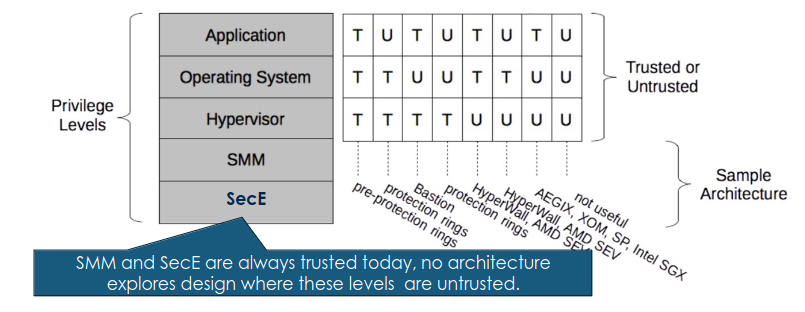
\includegraphics[width=0.7\textwidth]{img/hardware/ring trust.png}
    \caption{The trust relationship between the different components of the TCB}
  \end{figure}
  The protected software’s state is distributed throughout the processor. All of it needs to be
  protected from untrusted components and other (untrusted) protected software:
  \begin{itemize}
    \item the memory can be protected trough encryption and hashing of the data with integrity trees 
    \item the state needs to be flushed from the cores, and isolated into only one and any security
      modules(run only on secure cores)
    \item the state needs to also be isolated during I/O operations
  \end{itemize}

  Notice that key parts of the hardware TCB can be implemented as dedicated circuits or as firmware
  or other code running on dedicated processors. The former one is the most proposed academic 
  solution, but the latter one is whats actually implemented nowadays, example of this are the Intel
  ME and AMD PSP.\\

  Secure processor architectures ideally have no side effects, which are visible to the untrusted
  components whenever protected software is being executed. This is quite hard to achieve, so the
  effects of execution are erased when the program terminates or interrupts.
  \begin{subsection}{Protection inside the TEE}
    This whole architecture is based on \textit{trust}, which means that there is typically no
    protection from malicious TCB. Furthermore the software (code and data) executing within TEE
    protections is assumed to be benign and not malicious, as the system cannot protect software
    that is buggy or has vulnerabilities.\\
    \begin{boxH}
      Code bloat endangers the system, invalidating the assumptions about benign protected software.
      Attacks from within protected software should be defended. 
    \end{boxH}
  \end{subsection}
  \begin{subsection}{Ensuring Trustworthiness}
    The trustworthiness of the TCB depends on the ability to monitor the TCB code (hardware and
    software) execution as the system runs. TCB should be monitored to ensure it is trustworthy,
    which requires mechanisms to:
    \begin{itemize}
      \item Fingerprint and authenticate TCB code
      \item Monitor TCB execution
      \item Protect TCB code (on embedded security processor)
      \item Virtual Memory, ASLR, \dots
    \end{itemize}
  \end{subsection}
  \begin{subsection}{Root of Trust for TCB}
    Security of the system is derived from a root of trust.
    \begin{boxH}
      The \textbf{Root of Trust} is derived from a set of secret cryptographic keys only accessible
      from the TCB components, from which further keys can be derived.
    \end{boxH}
    The keys can be either:
    \begin{itemize}
      \item Burn in at the factory by the manufacturer (but implies trust issues with the
        manufacturer and the supply chain)
      \item Derived from Physically Unclonable Functions (but require reliability and extra hardware
        to derive keys from PUF)
    \end{itemize}

    We could say that the root of trust is derived from a signing key and a verification one:
    \begin{itemize}
      \item The signing key is used to encrypt the data sent to the processor
        \begin{itemize}
          \item this key also allows to "\textit{measure}" the code inside the TEE to attest to the
            external users what code is actually running
        \end{itemize}
      \item The verification key is used to verify the data sent to the processor
    \end{itemize}
    Because it uses an asymmetric encryption scheme, it needs an infrastructure to manage the keys.
  \end{subsection}
\end{section}
\begin{section}{System Memory Protection}
  Memory is vulnerable to different types of attacks:
  \begin{itemize}
    \item Untrusted software running no the processor
    \item Physical attacks on the memory bus, other devices snooping on the bus, man-in-the- middle attacks with malicious device
    \item Physical attacks on the memory (Coldboot, \dots)
    \item Malicious devices using DMA or other attacks
  \end{itemize}
  but in general, those attacks can be categorized as follows:
  \begin{itemize}
    \item \textbf{Snooping}: reading data content passively
    \item \textbf{Spoofing}: injecting new memory commands to try to read or modify data
    \item \textbf{Splicing}: combine portions of legitimate memory commands into new memory commands
      to read or modify data.
    \item \textbf{Replay}: replaying memory commands to read or modify data
    \item \textbf{Disturbance}: DoS on memory bus, repeated memory accesses to age circuits,
      repeated access to make Rowhammer, etc
  \end{itemize}
  
  \begin{subsection}{Protecting Confidentiality}
    Contents of the memory can be protected with encryption: data going out of the CPU is encrypted,
    and data coming from memory is decrypted before CPU use.
    For this purpose we use 2 engines: an encryption engine (usually AES in CTR mode) encrypts data
    going out of the processor chip, and a decryption engine decrypts data coming from memory.

    \begin{figure}[H]
      \centering
      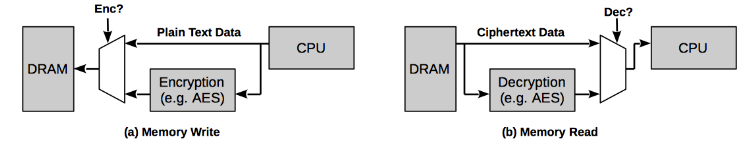
\includegraphics[width=0.7\textwidth]{img/hardware/memory confidentiality.png}
      \caption{Memory confidentiality protection}
    \end{figure}
  \end{subsection}

  \begin{subsection}{Protecting Integrity}
    Integrity can be protected with hashing, and in particular with hash trees. A hash tree (also
    called Merkle Tree) is a logical tree structure, typically a binary tree, where two child nodes
    are hashed together to create a parent node. The root node is a hash that depends on the value
    of all the leaf nodes.

    \begin{figure}[H]
      \centering
      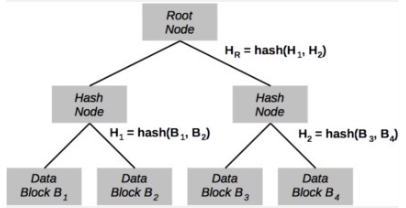
\includegraphics[width=0.5\textwidth]{img/hardware/merkle tree.png}
      \caption{The structure of a Merkle Tree}
    \end{figure}
    Message Authentication Codes (MACs) can be used instead of hashes, and a smaller “Bonsai” tree
    can be constructed.
    \begin{figure}[H]
      \centering
      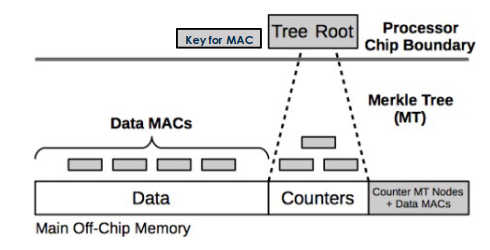
\includegraphics[width=0.5\textwidth]{img/hardware/bonsai hash tree.png}
      \caption{The structure of a Bonsai Tree}
    \end{figure}

    The integrity tree needs to consider the region of memory to protect:
    \begin{itemize}
      \item the whole memory
      \item parts of memory (e.g., per application, VM, etc.)
      \item the external storage (e.g., data swapped to disk)
    \end{itemize}
  \end{subsection}

  \begin{subsection}{Access Pattern Protection}
    Snooping attacks can target extracting data (protected with encryption) or extracting access
    patterns to learn what a program is doing.\\
    Access patterns (traffic analysis) attacks can be protected using \textbf{Oblivious RAM}, such
    as Path ORAM. This is on top of encryption and integrity checking.

    \begin{figure}[H]
      \centering
      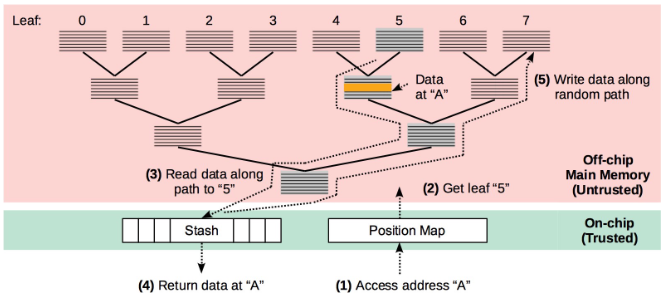
\includegraphics[width=0.5\textwidth]{img/hardware/access pattern protection.png}
      \caption{The structure of a Path ORAM}
    \end{figure}

  \end{subsection}

  \begin{subsection}{Security of Non-Volatile Memories and NVRAMs}
    Non-volatile memories (NVMs) can store data even when there is no power. Non-volatile
    random-access memory NVRAM) are a specific type of NVM that is suitable to serve as a computer
    system’s main memory and replace or augment DRAM.
    There are many types of NVRAMs:
    \begin{itemize}
      \item ReRAM – based on memristors, stores data in the resistance of a dielectric material
      \item FeRAM – uses ferroelectric material instead of a dielectric material
      \item MRAM – uses ferromagnetic materials and stores data in the resistance of a storage cell
      \item PCM – typically uses chalcogenide glass, where different glass phases have different resistances
    \end{itemize}
    With this technologies, some security considerations are due:

    \begin{itemize}
      \item Data remanence makes passive attacks easier (e.g., data extraction)
      \item Data is maintained after reboot or crash (security state also needs to be correctly
        restored after reboot or crash)
    \end{itemize}

    To protect the integrity of the data stored in NVRAMs, an integrity tree can be used, but 
    the atomicity of memory updates and its granularity(which data is persisted) need to be
    considered.\\
  \end{subsection}
  To wrap it up, here's a summary list:
  \begin{itemize}
    \item Encryption – snooping and spoofing protection
    \item Hashing – spoofing, splicing, replay (counters must be used), and disturbance
    protection
    \item Oblivious Access – snooping protection
  \end{itemize}

\end{section}

\begin{section}{Multiprocessor and Many-Core protection}
  Symmetric Multi-Processing (SMP) and Distributed Share Memory (DSM), also referred to as
  Non-Uniform Memory Access (NUMA), offer two ways of connecting many CPUs. In particular each core
  is untrusted by any other by default, except itself, as any other element(routers, connectors,
  \dots).

  \begin{figure}[H]
    \centering
    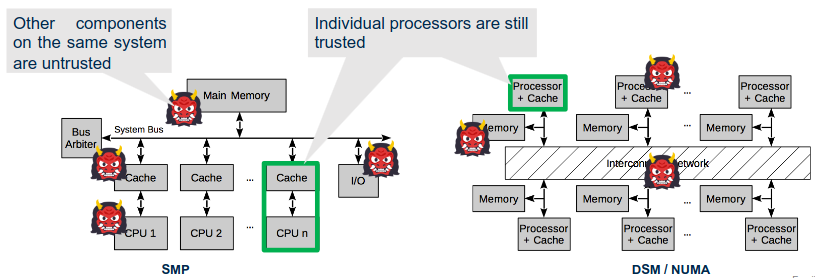
\includegraphics[width=0.7\textwidth]{img/hardware/smp and dsm.png}
    \caption{Comparison between SMP and NUMA}
  \end{figure}

  \begin{subsection}{SMP Protections}
    SMP refers to the computer architecture where multiple identical cores are interconnected
    to a single shared main memory, with full accessibility to all the I/O devices.\\
    In this architecture the bus is untrusted, for this reason the traffic could be encrypted
    between processors, by sharing an hard-coded key between each pair of processors, or by
    distributing keys using a public key infrastructure.\\
    To ensure the integrity of the messages, MACs can be used, while to protect the memory merkle
    tree can be implemented, either shared or per processor.
  \end{subsection}

  \begin{subsection}{DSM/NUMA Protection}
    DSM is a mechanism that manages memory across multiple nodes and makes inter-process
    communications transparent to end-users.

    \begin{figure}[H]
      \centering
      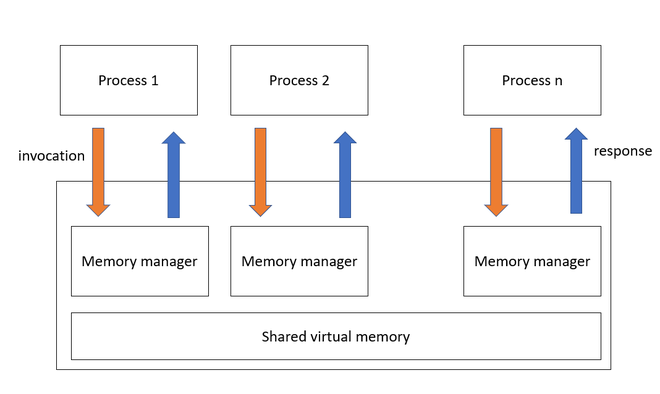
\includegraphics[width=0.7\textwidth]{img/hardware/DMS example.png}
      \caption{Example of how the DSM works}
    \end{figure}
    In a specular way to SMP, to ensure confidentiality, encryption can be used, and integrity can
    be ensured with MACs.\\
    The real difference lies in the memory protection: while with SMP the bus can be snooped to
    alter the memory tree, this is not possible anymore because DSM is usually point to point.

  \end{subsection}
  \begin{subsection}{Protected Inter-processor Communication}
    In addition to the existing assumption about protected memory communication, designs with
    multiple processors or cores assume the inter- processor communication will be protected:
    \begin{itemize}
      \item Confidentiality
      \item Integrity
      \item Communication pattern protection
    \end{itemize}
  \end{subsection}

  \begin{subsection}{Performance Challenges}
    Interconnects between processors are very fast, for example HyperTransport specifies speeds over
    50 GB/s, and with AES with block size 128 bits, it would mean that just for encryption we would
    need 3 billion (giga) AES block encryptions or decryption per second.\\
    Using counter mode could speed things up, but it would need to know or predict the counters, and
    still generate the pads in time.
  \end{subsection}
\end{section}
